%!TEX root = ../prueba.tex
\section{Introducción}

En el capítulo anterior se identificó un problema, se enlistaron sus causas y consecuencias. En este capítulo se describirá lo que el equipo propone para resolver este problema utilizando diagramas bajo la especificación de \textit{UML} del \textit{Business Process Modeling} y la visión del proyecto, la cual se presenta a continuación.\\

{\em{Diseñar e implementar un sistema que mejore el tiempo de respuesta de una cafetería para atender pedidos a clientes en horas de alta concurrencia.\\}}

\section{Descripción de la Propuesta}
El diagrama que se muestra en la figura \ref{fig:bpmn} muestra las actividades o tareas que deberá realizar cada actor del sistema para que se cumpla con la visión del proyecto. A continuación se enlistan estas tareas y se hace una descripción breve de qué consisten, cabe mencionar que el flujo de este diagrama es el ideal. También es pertinente hacer la observación de que este flujo es para aquellos pedidos que requieren ser atendidos por la cocina del local y que ya han sido pagados por una de las formas de pago disponibles. Si el contenido del pedido es únicamente de abarrotes no es requerido notificar a la cocina y sólo se procede a realizar el pago de forma habitual.

\begin{figure}[hbtp!]
	\begin{center}
		\fbox{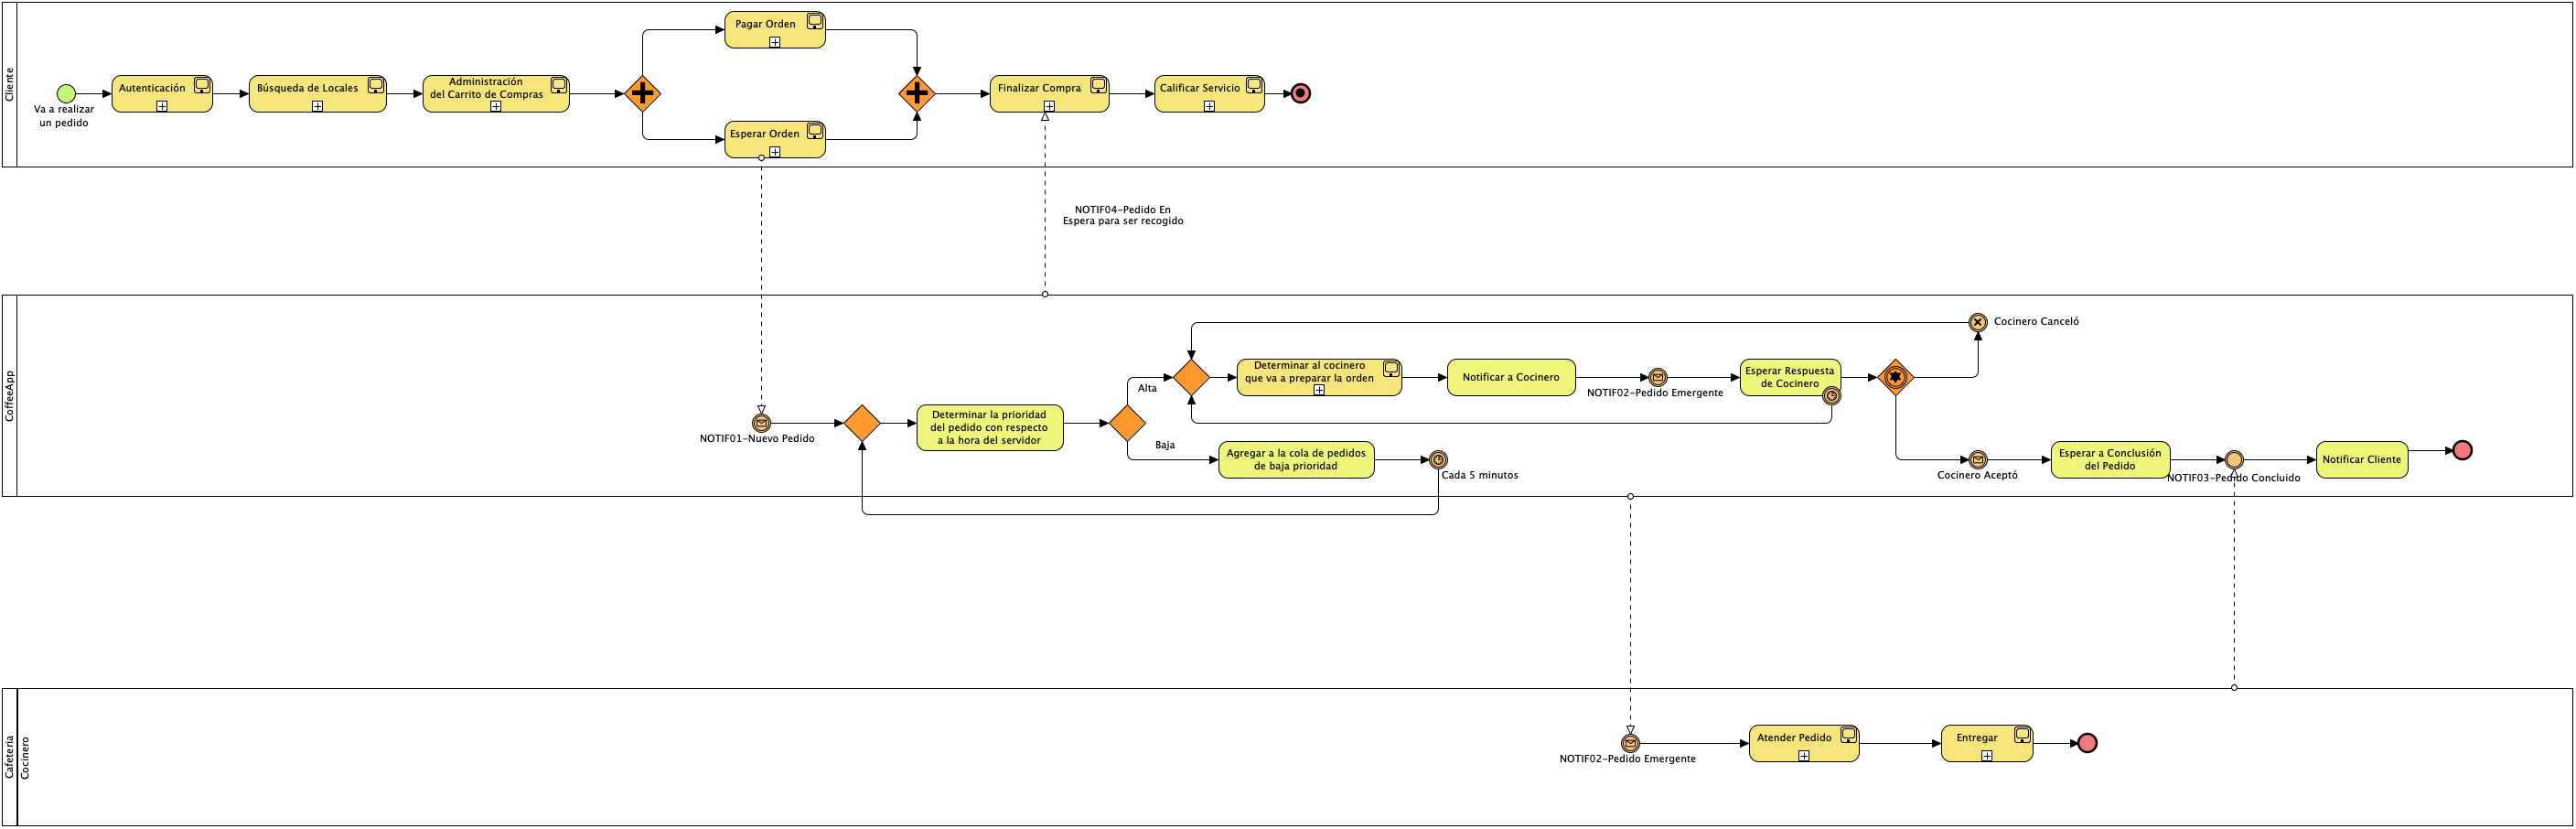
\includegraphics[width=\textheight,angle=90]{img/PropuestaDeSolucion}}
		\caption{Propuesta de Solución}
		\label{fig:bpmn}
	\end{center}
\end{figure}

\begin{description}
	\item[Cliente:]\hspace{1pt}
		
		\begin{enumerate}
			\item \label{PROC01Cliente:inicio} \init El proceso inicia cuando el cliente va a utilizar la aplicación móvil. Continúa el sub proceso de autenticación en el paso \ref{PROC01Cliente:autenticacion}.
			\item \label{PROC01Cliente:autenticacion}\process En el proceso de autenticación el cliente iniciará sesión en la aplicación móvil o en su defecto se registrará. Continúa con el paso \ref{PROC01Cliente:consultarLocales}
			\item \label{PROC01Cliente:consultarLocales}\task El dispositivo móvil desde el cual el cliente inicia sesión le proporciona a la aplicación móvil una ubicación geográfica aproximada, la aplicación móvil le desplegará en pantalla al cliente los locales más cercanos a su posición en un radio aproximado de 2 kilómetros. Continúa con el paso \ref{PROC01Cliente:seleccionarLocal}.
	\item \label{PROC01Cliente:seleccionarLocal} \task El cliente selecciona un local de su preferencia ya sea de los desplegados en el paso \ref{PROC01Cliente:consultarLocales} o utilizando la aplicación para buscar un local en particular. Continúa con el paso \ref{PROC01Cliente:consultarListaDeProductos}.
			\item \label{PROC01Cliente:consultarListaDeProductos}\task El cliente indica que va a comprar uno o más productos consulta la lista de productos disponibles del local seleccionado en el paso \ref{PROC01Cliente:seleccionarLocal}. Continúa con el paso \ref{PROC01Cliente:administrarCarritoDeCompras}.
			\item \label{PROC01Cliente:administrarCarritoDeCompras}\process El cliente seleccionará los productos que va a comprar en la aplicación móvil. Continúa con el paso \ref{PROC01Cliente:indicarTipo}. En este proceso se especificará el método de pago así como la posibilidad de agregar notas adicionales a los productos solicitados que así el cliente lo requiera.
			\item \label{PROC01Cliente:indicarTipo} \task El cliente indicará en la aplicación si su pedido debe ser enviado de forma inmediata a la cocina o se debe enviar en una hora en particular.
			\item \label{PROC01Cliente:gateUno} \gate Si el pedido del cliente es del tipo inmediato se continúa con el paso \ref{PROC01Cliente: confirmarPedido}, en caso de que el pedido del cliente sea de tipo programado se continúa con el paso \ref{PROC01Cliente:indicarHora}. 
			\item \label{PROC01Cliente:indicarHora} \task El cliente indicará la hora en la que quiere que su pedido llegue a la cocina para ser atendido por algún cocinero. Continúa con el paso \ref{PROC01Cliente:confirmarPedido}.
			\item \label{PROC01Cliente:confirmarPedido} \task El cliente indicará a la aplicación que va a ir al local seleccionado para recoger su pedido. 
			\item \label{PROC01Cliente:notif} Cuando el pedido del cliente ha sido preparado y empaquetado para su recepción el cliente irá al local seleccionado y recogerá su pedido y concluye el flujo.
		\end{enumerate}
	
	\item[Coffee App:]\hspace{1pt}
		\begin{enumerate}
			\item \label{PROC01App:ValidarExistencia}\task La aplicación móvil deberá validar la existencia de los productos contenidos en el carrito de compras en el local que el cliente haya seleccionado para realizar su pedido.
			\item \label{PROC01App:notif} La aplicación recibe y atiende la notificación de un nuevo pedido ejercida por un cliente y continúa con el paso \ref{PROC01App:servidor}.	
			\item \label{PROC01App:servidor} \task Si la prioridad de el pedido es alta, es decir el tipo del pedido es inmediato se debe continuar con el paso \ref{PROC01App:notificarCocina}. En caso contrario, el pedido es de tipo programadom, por lo que el pedido pasará a formar parte de una estructura de datos que será revisada por otro proceso, el cual determinará si el pedido debe ser notificado a la cocina o continuar en espera.
			\item \label{PROC01App:notificarCocina} \task Cuando la prioridad de un pedido es alta se mandará una notificación a los cocineros que estén disponibles en local para ser atendida.
			\item \label{PROC01App:atencionPedido} Cuando un cocinero ha seleccionado atender un pedido la aplicación recibe la notificación correspondiente y continúa con el paso \ref{PROC01App:horaDeAtencion}.
			\item \label{PROC01App:horaDeAtencion} \task La aplicación móvil calculará la hora aproximada en la que el cocinero atenderá el pedido con base en sus pedidos anteriores. Continúa con el paso \ref{PROC01App:calcularHoraFinalizacion}.
			\item \label{PROC01App:calcularHoraFinalizacion} \task La aplicación móvil calculará la hora aproximada en la que el cocinero concluirá la preparación del pedido. Continúa con el paso \ref{PROC01App:notificarCliente}.
			\item \label{PROC01App:notificarCliente} \task La aplicación móvil le notificará al cliente la hora aproximada en la que podrá ir al local a recoger su pedido.
			\item \label{PROC01App:pedidoNoEntregado} Cuando un pedido no ha sido recogido en el lapso de 15 minutos la aplicación mandará una notificación a los clientes que hayan realizado al menos una compra en ese local para recoger y realizar el pago correspondiente por el pedido.
		\end{enumerate}

	\item[Cocinero:]\hspace{1pt}
		\begin{enumerate}
			\item \label{PROC01Cocinero:notif} Una vez que se ha determinado que un pedido tiene prioridad alta se notificará a la cocina para que un cocinero atienda el pedido. Continúa con el paso \ref{PROC01Cocinero:seleccionarPedido}.
			\item \label{PROC01Cocinero:seleccionarPedido} \task El cocinero selecciona el pedido emergente para indicar que lo va a atender. Cuando un pedido emergente no ha sido seleccionado por algún cocinero, se le notificará al cliente que hay un retraso aproximado de 5 minutos para atender su orden, más sin en cambio un cocinero indica que vas a atender un pedido el sistema realizará los cálculos correspondientes para determinar el tiempo estimado de entrega. Continúa con el paso \ref{PROC01Cocinero:atender}.
			\item \label{PROC01Cocinero:atender} \task El cocinero atiende el pedido preparándolo. Continúa con el paso \ref{PROC01Cocinero:espera}.
			\item \label{PROC01Cocinero:espera} \task Una vez el cocinero indicó que ha concluido de preparar el pedido del cliente, la aplicación comenzará a tomar el tiempo para que el cliente pase al local correspondiente a recoger su pedido. Si el cliente llegó en un lapso menor a 15 minutos se continúa con el paso \ref{PROC01Cocinero:entrega},en caso contrario se continúa con el paso \ref{PROC01Cocinero:oferta}.
			\item  \label{PROC01Cocinero:entrega} \task Cuando el cliente llegó en el rango de tiempo de 0 a 15 minutos se le hará entrega de su pedido y finaliza el proceso.
			\item \label{PROC01Cocinero:oferta} \task Cuando el cliente no llegó en el rango de tiempo de 0 a 15 minutos el cocinero indicará que el pedido puede ser tomado por otro cliente que pague por él en un tiempo limitado de 15 minutos. Continúa con el paso \ref{PROC01Cocinero:entrega}.
		\end{enumerate}

\end{description}


\section{Arquitectura Física}

En esta sección se realizar la especificación técnica y física de la arquitectura sobre la cual la aplicación y el sistema funcionaran desde su puesta en producción. Dicha especificación se realiza utilizando como base la figura \ref{fig:arqFisica}.

\begin{figure}[hbtp!]
	\begin{center}
		\fbox{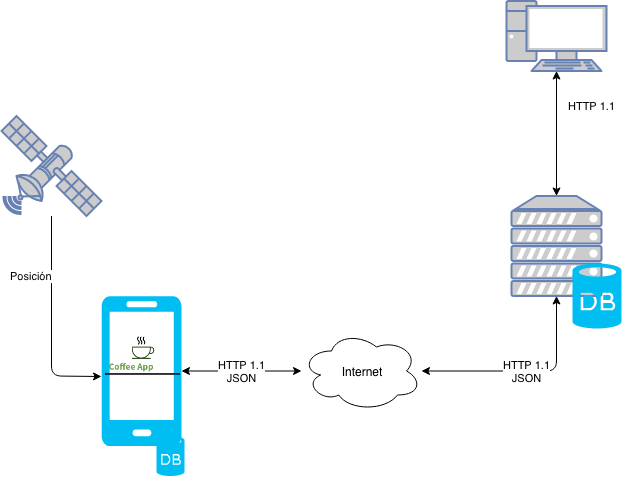
\includegraphics[width=.5\textwidth]{img/arqFisica}}
		\caption{Arquitectura Física del Sistema}
		\label{fig:arqFisica}
	\end{center}
\end{figure}

\subsection{Arquitectura Base}
El sistema está pensado para trabajar bajo un esquema centralizado tomando como base la arquitectura \textbf{Cliente-Servidor}. Esta arquitectura nos sirve como punto de partida debido a dos principales razones:
	\begin{itemize}
		\item Es requerido un punto centralizado(servidor) donde se almacene la mayor cantidad de información y que sea un punto de acceso para varios dispositivos.
		\item Es requerido hacer la implementación de dos diferentes clientes desde los cuales se tendrá acceso al servidor y por consiguiente a la información. El primer cliente consta de una aplicación móvil para dispositivos con sistema operativo Android, el segundo cliente consta de una aplicación web basada en \textit{Servlets} y \textit{JSP's}. 
	\end{itemize}

Se optó también por utilizar como base la arquitectura \textbf{Cliente - Servidor} ya que nos permite el uso del protocolo \textit{HTTP 1.1} para crear varios canales de comunicación entre los distintos clientes que accederán al sistema. El protocolo \textit{HTTP} nos define que para que exista comunicación entre el Cliente y el Servidor se debe hacer uso de dos mecanismos: una \textit{Petición} y una \textit{Respuesta}. A grandes rasgos, la petición está formada entre otras cosas por cabeceras, métodos y parámetros los cuales son enviados desde el cliente a través de la red hasta llegar al servidor el cual debe validar que la \textit{URL} desde la cual se hace la petición es válida. Posteriormente el servidor procesa la petición y en caso de existir el recurso y el método contenido en la petición le devolverá al cliente una respuesta con la información solicitada utilizando el formato indicado en el \textit{MIME/TYPE} de la respuesta.\\

Los actores que podrán acceder al sistema mediante la aplicación web son:
	\begin{itemize}
		\item El \getElementById[Stakeholder]{Jefe} dado que es el encargado de registrar, editar o eliminar la información de las cafeterías de las que es dueño así como sus respectivos locales y productos que se podrán encontrar en todos los locales de su franquicia.
		\item El \getElementById[Stakeholder]{Administrador} dado que es el encargado de habilitar el acceso a las personas que tienen una cuenta bloqueada al sistema.
		\item El \getElementById[Stakeholder]{ResponsableDeLocal} dado que es el encargado de registrar la información de los productos que se ofertan en un local.
	\end{itemize}

Los actores que tendrán acceso a la aplicación móvil son:
	\begin{itemize}
		\item El \getElementById[Stakeholder]{Cliente} dado que desde su dispositivo únicamente podrá consultar información de las cafeterias, locales y productos publicados para realizar pedidos que serán atendidos por el personas de los locales, la aplicación móvil hará uso de dos mecanismos relevantes:
		\begin{itemize}
			\item El módulo GPS ya que cuando el cliente acceda a la aplicación se determinará su posición y con esto la ubicación de los locales más cercanos en un radio de 2 kilómetros.
			\item Una base de datos local que almacenará los pedidos que no han sido confirmados para que el cocinero de un local inicie su preparación.
		\end{itemize}
		\item El \getElementById[Stakeholder]{Cocinero} dado que a su tableta o a la tableta proporcionada por la cafetería, atenderá los pedidos e indicará la conclusión de su preparación para que se le entrege al cliente.
\end{itemize}


\subsection{Especificaciones Técnicas}
A continuación se especifican los detalles técnicos del sistema, es decir, el Hardware y Software requerido para que el sistema opere de forma estable.

\subsubsection{Servidor}
El servidor tiene las siguientes especificaciones:
	\begin{description}
		\item[Marca:]Servidor Dell PowerEdge T30.
		\item[Procesador:]Intel Xeon E3-1225V5 3.30GHz.
		\item[Memoria RAM:]8GB DDR4.
		\item[Disco Duro:]1TB.
		\item[Sistema Operativo:] CentOS 7.4-1708.
	\end{description}

\subsection{Base de Datos}
	\begin{description}
		\item[SGBD:] Postgresql 9.4
	\end{description}

\subsubsection{Cliente Web}
La aplicación web puede ser utilizada bajo las siguientes especificaciones:
	\begin{description}
		\item[Navegadores Compatibles:]\hspace{0.5pt}
			\begin{itemize}
				\item Google Chrome Versión $\geq$ 70.0.3538.
				\item Mozilla Firefox $\geq$ 63.0.
				\item Safari $\geq$ 12.0.
			\end{itemize}
		\item[Resolución:]\hspace{0.5pt}
			\begin{itemize}
				\item Mínima:1027x768
				\item Máxima:1920x1080
			\end{itemize}
	\end{description}

\subsubsection{Cliente Móvil}
La aplicación móvil puede ser utilizada bajo las siguientes especificaciones:
	\begin{description}
		\item[Sistema Operativo:] Android >= 5.0 Lollipop.
		\item[Memoria RAM:] 2GB.
		\item[Almacenamiento:] 16 GB.
	\end{description}


\section{Arquitectura Lógica}
Una vez descrita la arquitectura física del sistema, es requerido indicar y especificar cómo será construido. En general las aplicaciones que se van a desarrollar utilizarán una arquitectura a capas. En la figura \ref{fig:arqLogica} se pueden observar las capas del sistema en los diferentes clientes(o aplicaciones) y posteriormente se hará una descripción de la función de cada capa.

\begin{figure}[hbtp!]
	\begin{center}
		\fbox{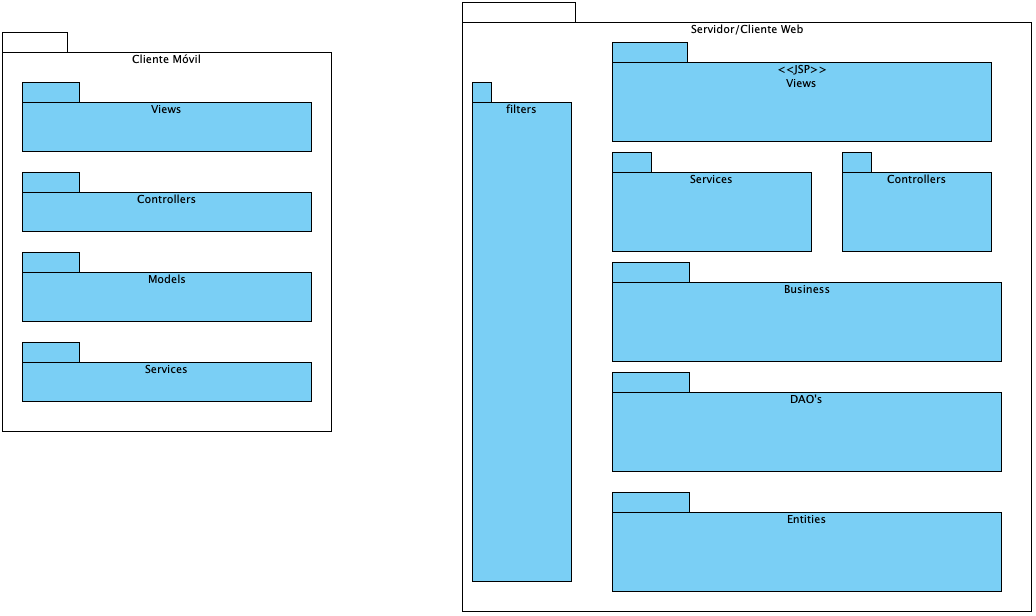
\includegraphics[width=0.8\textwidth]{img/arqLogicaP}}
		\caption{Arquitectura Lógica del Sistema}
		\label{fig:arqLogica}
	\end{center}
\end{figure}

\subsection{Arquitectura Lógica del Servidor/Aplicación Web}
Como se mencionó al iniciar esta sección, las aplicaciones están construidas a partir de una arquitectura multi capa.El servidor(paquete del lado derecho en la figura \ref{fig:arqLogica}) está dividido en las siguientes capas:
	\begin{description}
		\item[Entities:] En esta capa se definen las clases que se utilizarán para la manipulación de las estructuras de datos de la base de datos.
		\item[DAO's:] En esta capa se definen las clases que sirven de interacción entre la capa de \textit{business} y la capa de \textit{entities} para la recolección de datos utilizando el patrón de diseño DAO.
		\item[Business:] En esta capa se definen las clases que sirven para la abstracción de las reglas de negocio así como de las operaciones y funciones disponibles en el sistema.
		\item[Services:] En esta capa se definen las clases que corresponden al servicio RESTful que será consumido por la aplicación móvil.
		\item[Controllers:] Está capa tiene el propósito establecido para la capa de \textit{Controlador} en el patrón de diseño \textit{MVC} en donde se va a administrar el flujo de datos que hay entre la capa \textit{views} y la capa \textit{business}.
		\item[Views:] Está capa contiene los archivos JPA's que presentan las interfaces de usuario para la aplicación web.
	\end{description}
	
\subsection{Arquitectura Lógica de la Aplicación Móvil}
La aplicación móvil se va a construir con base en el patrón arquitectónico \textit{MVC}, agregando una capa la cual tiene como principal propósito administrar las peticiones que se van a mandar al servidor y proveer de datos a la capa de \textit{Models}. Así mismo dado que la aplicación móvil es nativa del sistema operativo Android, se hará uso de algunos patrones de diseño establecidos por \textit{Google} para el comportamiento de algunos componentes como lo es el patrón \textit{Adapter} para el componente \textit{Recycler View}.




